\PassOptionsToPackage{unicode=true}{hyperref} % options for packages loaded elsewhere
\PassOptionsToPackage{hyphens}{url}
%
\documentclass[]{article}
\usepackage{lmodern}
\usepackage{amssymb,amsmath}
\usepackage{ifxetex,ifluatex}
\usepackage{fixltx2e} % provides \textsubscript
\ifnum 0\ifxetex 1\fi\ifluatex 1\fi=0 % if pdftex
  \usepackage[T1]{fontenc}
  \usepackage[utf8]{inputenc}
  \usepackage{textcomp} % provides euro and other symbols
\else % if luatex or xelatex
  \usepackage{unicode-math}
  \defaultfontfeatures{Ligatures=TeX,Scale=MatchLowercase}
\fi
% use upquote if available, for straight quotes in verbatim environments
\IfFileExists{upquote.sty}{\usepackage{upquote}}{}
% use microtype if available
\IfFileExists{microtype.sty}{%
\usepackage[]{microtype}
\UseMicrotypeSet[protrusion]{basicmath} % disable protrusion for tt fonts
}{}
\IfFileExists{parskip.sty}{%
\usepackage{parskip}
}{% else
\setlength{\parindent}{0pt}
\setlength{\parskip}{6pt plus 2pt minus 1pt}
}
\usepackage{hyperref}
\hypersetup{
            pdftitle={Introduction to MethICA},
            pdfauthor={Lea Meunier},
            pdfborder={0 0 0},
            breaklinks=true}
\urlstyle{same}  % don't use monospace font for urls
\usepackage[margin=1in]{geometry}
\usepackage{color}
\usepackage{fancyvrb}
\newcommand{\VerbBar}{|}
\newcommand{\VERB}{\Verb[commandchars=\\\{\}]}
\DefineVerbatimEnvironment{Highlighting}{Verbatim}{commandchars=\\\{\}}
% Add ',fontsize=\small' for more characters per line
\usepackage{framed}
\definecolor{shadecolor}{RGB}{248,248,248}
\newenvironment{Shaded}{\begin{snugshade}}{\end{snugshade}}
\newcommand{\AlertTok}[1]{\textcolor[rgb]{0.94,0.16,0.16}{#1}}
\newcommand{\AnnotationTok}[1]{\textcolor[rgb]{0.56,0.35,0.01}{\textbf{\textit{#1}}}}
\newcommand{\AttributeTok}[1]{\textcolor[rgb]{0.77,0.63,0.00}{#1}}
\newcommand{\BaseNTok}[1]{\textcolor[rgb]{0.00,0.00,0.81}{#1}}
\newcommand{\BuiltInTok}[1]{#1}
\newcommand{\CharTok}[1]{\textcolor[rgb]{0.31,0.60,0.02}{#1}}
\newcommand{\CommentTok}[1]{\textcolor[rgb]{0.56,0.35,0.01}{\textit{#1}}}
\newcommand{\CommentVarTok}[1]{\textcolor[rgb]{0.56,0.35,0.01}{\textbf{\textit{#1}}}}
\newcommand{\ConstantTok}[1]{\textcolor[rgb]{0.00,0.00,0.00}{#1}}
\newcommand{\ControlFlowTok}[1]{\textcolor[rgb]{0.13,0.29,0.53}{\textbf{#1}}}
\newcommand{\DataTypeTok}[1]{\textcolor[rgb]{0.13,0.29,0.53}{#1}}
\newcommand{\DecValTok}[1]{\textcolor[rgb]{0.00,0.00,0.81}{#1}}
\newcommand{\DocumentationTok}[1]{\textcolor[rgb]{0.56,0.35,0.01}{\textbf{\textit{#1}}}}
\newcommand{\ErrorTok}[1]{\textcolor[rgb]{0.64,0.00,0.00}{\textbf{#1}}}
\newcommand{\ExtensionTok}[1]{#1}
\newcommand{\FloatTok}[1]{\textcolor[rgb]{0.00,0.00,0.81}{#1}}
\newcommand{\FunctionTok}[1]{\textcolor[rgb]{0.00,0.00,0.00}{#1}}
\newcommand{\ImportTok}[1]{#1}
\newcommand{\InformationTok}[1]{\textcolor[rgb]{0.56,0.35,0.01}{\textbf{\textit{#1}}}}
\newcommand{\KeywordTok}[1]{\textcolor[rgb]{0.13,0.29,0.53}{\textbf{#1}}}
\newcommand{\NormalTok}[1]{#1}
\newcommand{\OperatorTok}[1]{\textcolor[rgb]{0.81,0.36,0.00}{\textbf{#1}}}
\newcommand{\OtherTok}[1]{\textcolor[rgb]{0.56,0.35,0.01}{#1}}
\newcommand{\PreprocessorTok}[1]{\textcolor[rgb]{0.56,0.35,0.01}{\textit{#1}}}
\newcommand{\RegionMarkerTok}[1]{#1}
\newcommand{\SpecialCharTok}[1]{\textcolor[rgb]{0.00,0.00,0.00}{#1}}
\newcommand{\SpecialStringTok}[1]{\textcolor[rgb]{0.31,0.60,0.02}{#1}}
\newcommand{\StringTok}[1]{\textcolor[rgb]{0.31,0.60,0.02}{#1}}
\newcommand{\VariableTok}[1]{\textcolor[rgb]{0.00,0.00,0.00}{#1}}
\newcommand{\VerbatimStringTok}[1]{\textcolor[rgb]{0.31,0.60,0.02}{#1}}
\newcommand{\WarningTok}[1]{\textcolor[rgb]{0.56,0.35,0.01}{\textbf{\textit{#1}}}}
\usepackage{graphicx,grffile}
\makeatletter
\def\maxwidth{\ifdim\Gin@nat@width>\linewidth\linewidth\else\Gin@nat@width\fi}
\def\maxheight{\ifdim\Gin@nat@height>\textheight\textheight\else\Gin@nat@height\fi}
\makeatother
% Scale images if necessary, so that they will not overflow the page
% margins by default, and it is still possible to overwrite the defaults
% using explicit options in \includegraphics[width, height, ...]{}
\setkeys{Gin}{width=\maxwidth,height=\maxheight,keepaspectratio}
\setlength{\emergencystretch}{3em}  % prevent overfull lines
\providecommand{\tightlist}{%
  \setlength{\itemsep}{0pt}\setlength{\parskip}{0pt}}
\setcounter{secnumdepth}{0}
% Redefines (sub)paragraphs to behave more like sections
\ifx\paragraph\undefined\else
\let\oldparagraph\paragraph
\renewcommand{\paragraph}[1]{\oldparagraph{#1}\mbox{}}
\fi
\ifx\subparagraph\undefined\else
\let\oldsubparagraph\subparagraph
\renewcommand{\subparagraph}[1]{\oldsubparagraph{#1}\mbox{}}
\fi

% set default figure placement to htbp
\makeatletter
\def\fps@figure{htbp}
\makeatother


\title{Introduction to MethICA}
\author{Lea Meunier}
\date{2020/07/21}

\begin{document}
\maketitle

\hypertarget{abstract}{%
\section{Abstract}\label{abstract}}

DNA methylation changes are widespread in human cancers, but the
underlying molecular mechanisms remain incompletely understood. We
developed an innovative statistical framework, MethICA, leveraging
independent component analysis to identify sources of DNA methylation
changes in tumors. The package includes a function that uses independent
component analysis to extract epigenetic signatures from methylation
data, as well as functions to calculate associations with sample
annotations and CpG characteristics. The package also provides
representations that facilitate the interpretation of methylation
components. This document, paired with the
``MethICA\_examples\_script.R'' demo script, outlines the typical
workflow for analyzing methylation signatures in a cancer series with
MethICA.

\hypertarget{package}{%
\section{Package}\label{package}}

Report issues at \url{https://github.com/FunGeST/MethICA}.

\newpage

\hypertarget{introduction}{%
\section{Introduction}\label{introduction}}

\hypertarget{installation-instructions}{%
\section{Installation Instructions}\label{installation-instructions}}

The latest version of the package can be installed from the FunGeST
GitHub repository using devtools:

\begin{Shaded}
\begin{Highlighting}[]
\KeywordTok{install.packages}\NormalTok{(}\StringTok{"devtools"}\NormalTok{)}
\KeywordTok{library}\NormalTok{(devtools)}
\NormalTok{devtools}\OperatorTok{::}\KeywordTok{install_github}\NormalTok{(}\StringTok{"FunGeST/MethICA"}\NormalTok{)}
\end{Highlighting}
\end{Shaded}

\hypertarget{dependencies}{%
\section{Dependencies}\label{dependencies}}

The R packages stringr, fastICA, cowplot, ggplot2, RColorBrewer, plotrix
and broom are required to perform MethICA analysis

\hypertarget{input-data}{%
\section{Input data}\label{input-data}}

Input files are necessary to perform the core MethICA analyses:

bval: methylation levels for each CpG or region (rows) in each sample
(columns)

CpG annotation: CpG table annotated with various (epi)genomic features

sample annotation: relevant sample annotations to interpret the
components

Please check the README file for detailed description of input files.
Examples are also provided with the package.

\hypertarget{load-methylation-data-and-annotations}{%
\subsection{Load methylation data and
annotations}\label{load-methylation-data-and-annotations}}

Once installed, load the package and you're ready to go!

\begin{Shaded}
\begin{Highlighting}[]
\CommentTok{# Load MethICA package}
\KeywordTok{library}\NormalTok{(MethICA)}
\KeywordTok{library}\NormalTok{(corrplot)}
\end{Highlighting}
\end{Shaded}

Define output directories.

\begin{Shaded}
\begin{Highlighting}[]
\CommentTok{# define output directory> }
\NormalTok{output.directory =}\StringTok{ "~/Test_MethICA/"}
\ControlFlowTok{if}\NormalTok{(}\OperatorTok{!}\KeywordTok{dir.exists}\NormalTok{(output.directory))\{}
  \KeywordTok{dir.create}\NormalTok{(output.directory)}
\NormalTok{\}}
\end{Highlighting}
\end{Shaded}

We provide example datasets from our hepatocellular carcinoma study
containing bval methylation table, annotation table and CpG feature for
liver data that can be loaded here:
\url{https://drive.google.com/drive/folders/1BTQOhvI_qQou1CD94N_TCV_TEbcBC671?usp=sharing}

\begin{Shaded}
\begin{Highlighting}[]
\CommentTok{# load example dataset> }
\NormalTok{data.directory <-}\StringTok{ "~/Downloads/MethICAdata/"}
\KeywordTok{load}\NormalTok{(}\KeywordTok{file.path}\NormalTok{(data.directory,}\StringTok{'LICAFR_methylation.Rdata'}\NormalTok{),}\DataTypeTok{verbose =}\NormalTok{ T)}
\end{Highlighting}
\end{Shaded}

Select the most variant CpG sites (based on standard deviation) for the
analysis.

\begin{Shaded}
\begin{Highlighting}[]
\CommentTok{# Select most variant CpG sites }
\NormalTok{NmostVar =}\StringTok{ }\DecValTok{100000}
\NormalTok{mysd <-}\StringTok{ }\KeywordTok{apply}\NormalTok{(bval,}\DecValTok{1}\NormalTok{,sd)}
\NormalTok{sel <-}\StringTok{ }\KeywordTok{order}\NormalTok{(mysd,}\DataTypeTok{decreasing=}\NormalTok{T)[}\DecValTok{1}\OperatorTok{:}\NormalTok{NmostVar]}
\CommentTok{# Reduce bval and CpG_feature matrix}
\NormalTok{bval <-}\StringTok{ }\NormalTok{bval[sel,];}\KeywordTok{dim}\NormalTok{(bval)}
\NormalTok{CpG_feature <-}\StringTok{ }\NormalTok{CpG_feature[}\KeywordTok{rownames}\NormalTok{(bval),]}
\end{Highlighting}
\end{Shaded}

\hypertarget{prepare-cpg-annotation-table}{%
\subsection{Prepare CpG annotation
table}\label{prepare-cpg-annotation-table}}

MethICA uses various (epi)genomic annotations of CpG sites to interpret
methylation components. Make sure you use correct annotations for the
tissue under study. For example, the CpG\_feature.Rdata file included in
the package corresponds the CpG annotation table of liver tissue used in
our hepatocellular carcinoma study. We provide the chromatin.feature
function to annotate your own CpG table. It requires different inputs
for each (epi)genomic feature that can be obtained from various sources.
For example, here are the links we used for our study:

file\_CGI : CpG island-based features (Island, Shore, Shelf, out of cgi)
from UCSC (not liver specific)

file\_genes : gene-based features (body, TSS500) from GENCODE
\url{https://www.gencodegenes.org/human/release_34lift37.html} (not
liver specific)

file\_chrom\_state : chromatin states defined from various histone marks
by the ROADMAP epigenomics project (liver specific)
\url{https://egg2.wustl.edu/roadmap/web_portal/chr_state_learning.html\#exp_18state}

file\_CpG\_context : methylation domains (HMD/PMD/LMR/UMR) defined from
WGBS data (liver specific)
\url{https://www.ncbi.nlm.nih.gov/geo/download/?acc=GSE113405\&format=file\&file=GSE113405\%5FLIV\%5FADLT\%2EMethylSeekR\%2Esegments\%2Ebed\%2Egz}

file\_replication : replication timing deciles obtained from Repli-Seq
data availbale on the ENCODE project data portal. Here we used Repli-Seq
from HepG2 cell line accessible under GEO accession number GSM923446
(liver specific)
\url{https://www.ncbi.nlm.nih.gov/geo/query/acc.cgi?acc=GSM923446}

The script used to extensively annotate CpG features
(feature\_table\_script.R) is provided in the RUNNING\_MethICA\_example
folder. It uses various types of (epi)genomic data (CpG islands, genes,
chromatin states, methylation domains) to annotate the tissue-specific
context of each CpG site.

\hypertarget{extract-methylation-components-with-ica}{%
\section{Extract methylation components with
ICA}\label{extract-methylation-components-with-ica}}

The mc.extract function performs independent component analysis (ICA)
and extracts methylation components from the methylation matrix.

input: bval methylation matrix

outputs: MC\_object with two matrices giving the contribution of CpGs
and samples to each component, and one vector giving components
stability. If compute\_stability = TRUE (recommended), mc.extract
performs n iterations of ICA, computes stability and selects the most
stable iteration,. If compute\_stability = FALSE, mc.extract performs a
single iteration of ICA and returns NA in stability vector

\begin{Shaded}
\begin{Highlighting}[]
\NormalTok{MC_object <-}\StringTok{ }\KeywordTok{mc.extract}\NormalTok{(bval, }\DataTypeTok{nb_comp =} \DecValTok{20}\NormalTok{, }\DataTypeTok{compute_stability =} \OtherTok{TRUE}\NormalTok{, }\DataTypeTok{nb_iteration =} \DecValTok{20}\NormalTok{, }\DataTypeTok{output.directory =}\NormalTok{ output.directory, }\DataTypeTok{save =} \OtherTok{TRUE}\NormalTok{)}
\end{Highlighting}
\end{Shaded}

Each methylation component (MC) is characterized by an activation
pattern across CpG sites and across samples. To interpret their
biological meaning, we first select the most contributing CpGs and
samples for each MC.

The mc.active.CpG function identifies CpGs with a contribution greater
than a defined threshold (method=``threshold'', recommended) or extracts
a defined number of most contributing CpGs (method=``number'').

The mc.active.sample function identifies the most contributing samples
(method=``absolute'') or those showing the greatest deviation from a set
of reference samples (method=``reference'').

\begin{Shaded}
\begin{Highlighting}[]
\CommentTok{# Extract the most contributing CpG sites for each MC}
\NormalTok{MC_contrib_CpG <-}\StringTok{ }\KeywordTok{mc.active.CpG}\NormalTok{(MC_object, }\DataTypeTok{method =} \StringTok{"threshold"}\NormalTok{)}

\CommentTok{# Extract the most contributing samples for each MC...}
\CommentTok{# based on absolute value of contribution }
\NormalTok{MC_active_sample =}\StringTok{ }\KeywordTok{mc.active.sample}\NormalTok{(MC_object, }\DataTypeTok{method =} \KeywordTok{c}\NormalTok{(}\StringTok{"absolute"}\NormalTok{, }\StringTok{"reference"}\NormalTok{)[}\DecValTok{1}\NormalTok{],}\DataTypeTok{bval =}\NormalTok{ bval , }\DataTypeTok{MC_contrib_CpG =}\NormalTok{ MC_contrib_CpG, }\DataTypeTok{number =} \KeywordTok{round}\NormalTok{(}\KeywordTok{nrow}\NormalTok{(MC_object}\OperatorTok{$}\NormalTok{Sample_contrib)}\OperatorTok{*}\FloatTok{0.1}\NormalTok{))}
\CommentTok{# or based on differential methylation level with reference sample (here normal samples)}
\NormalTok{MC_active_sample =}\StringTok{ }\KeywordTok{mc.active.sample}\NormalTok{(MC_object, }\DataTypeTok{method =} \KeywordTok{c}\NormalTok{(}\StringTok{"absolute"}\NormalTok{, }\StringTok{"reference"}\NormalTok{)[}\DecValTok{2}\NormalTok{],}\DataTypeTok{bval =}\NormalTok{ bval , }\DataTypeTok{MC_contrib_CpG =}\NormalTok{ MC_contrib_CpG, }\DataTypeTok{number =} \KeywordTok{round}\NormalTok{(}\KeywordTok{nrow}\NormalTok{(MC_object}\OperatorTok{$}\NormalTok{Sample_contrib)}\OperatorTok{*}\FloatTok{0.1}\NormalTok{), }\DataTypeTok{ref =} \KeywordTok{grep}\NormalTok{(}\StringTok{"N"}\NormalTok{, }\KeywordTok{colnames}\NormalTok{(bval), }\DataTypeTok{value =} \OtherTok{TRUE}\NormalTok{))}
\end{Highlighting}
\end{Shaded}

\hypertarget{represent-methylation-changes}{%
\section{Represent methylation
changes}\label{represent-methylation-changes}}

We then use the mc.change function to identify the major methylation
changes associated with each component. This function plots the average
methylation of the most contributing CpGs in the most contributing
samples versus reference samples. Examples below represent components
associated mostly with hypermethylation, hypomethylation or both. If
highly contributing samples include samples with high positive and
negative contributions, two distinct graphs are produced.

\begin{Shaded}
\begin{Highlighting}[]
\CommentTok{#Represent methylation changes in most contributing tumors vs. normal samples}
\KeywordTok{mc.change}\NormalTok{(MC_object, MC_active_sample, MC_contrib_CpG, bval, }\DataTypeTok{ref =} \KeywordTok{grep}\NormalTok{(}\StringTok{"N"}\NormalTok{, }\KeywordTok{colnames}\NormalTok{(bval), }\DataTypeTok{value =} \OtherTok{TRUE}\NormalTok{), }\DataTypeTok{output.directory =}\NormalTok{ output.directory)}
\end{Highlighting}
\end{Shaded}

Examples of outputs:
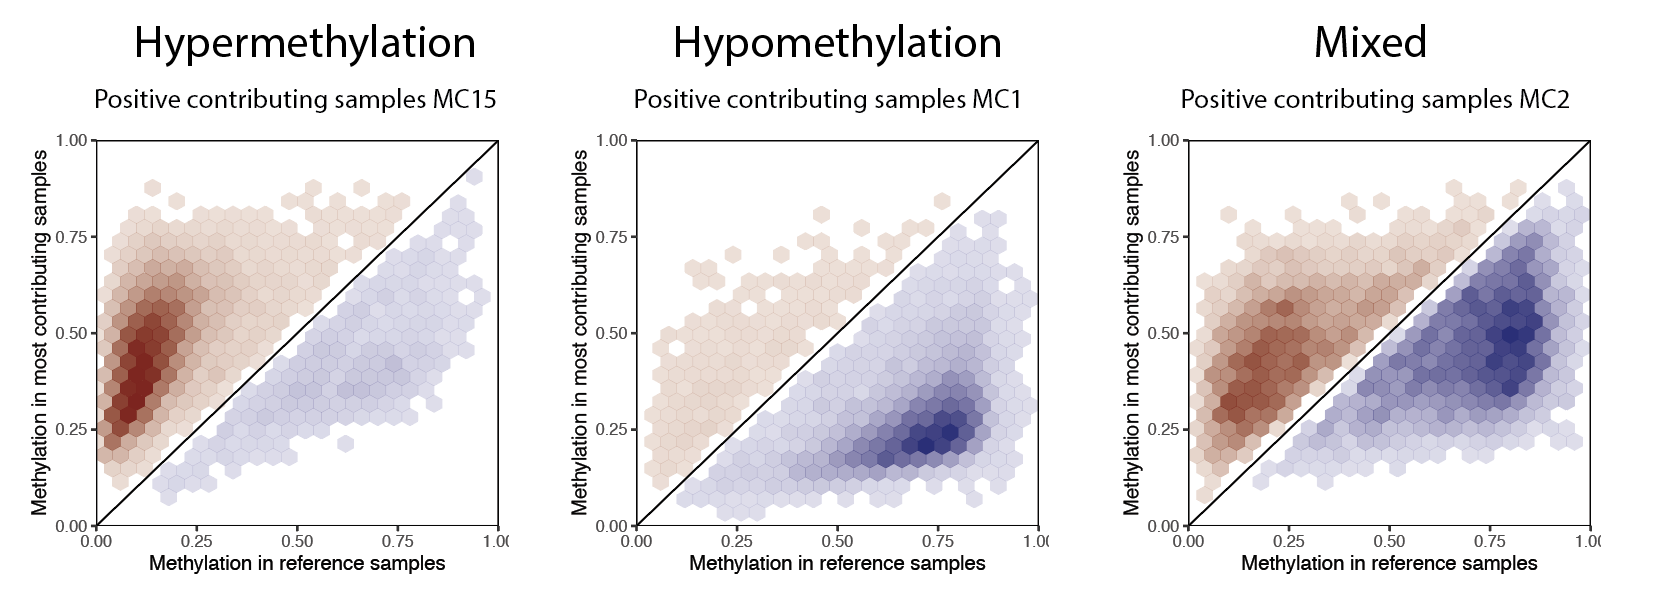
\includegraphics[width=1\textwidth,height=1\textheight]{./meth_change.png}

\hypertarget{explore-epigenomic-characteristics-of-the-most-contributing-cpgs}{%
\section{Explore epigenomic characteristics of the most contributing
CpGs}\label{explore-epigenomic-characteristics-of-the-most-contributing-cpgs}}

To better understand the components, we then explore the characteristics
of their most contributing CpGs. The enrich.CpG.feature function
computes enrichment scores of CpGs across epigenomic features from the
CpG\_feature table and generates various visual outputs. The example
below shows a hypermethylation component affecting preferentially CpG
sites located in CpG islands near transcription start sites, with
bivalent chromatin state. The ``other\_feature\_to\_test'' option of
enrich.CpG.feature function allows to compute enrichment and generate
barplots for any additional feature.

\begin{Shaded}
\begin{Highlighting}[]
\CommentTok{# Association of MCs with (epi)genomic characteristics}
\KeywordTok{enrich.CpG.feature}\NormalTok{(MC_object, MC_contrib_CpG, }\DataTypeTok{output.directory =}\NormalTok{ output.directory, }\DataTypeTok{CpG_feature =}\NormalTok{ CpG_feature)}
\end{Highlighting}
\end{Shaded}

Example of outputs for MC5 component:
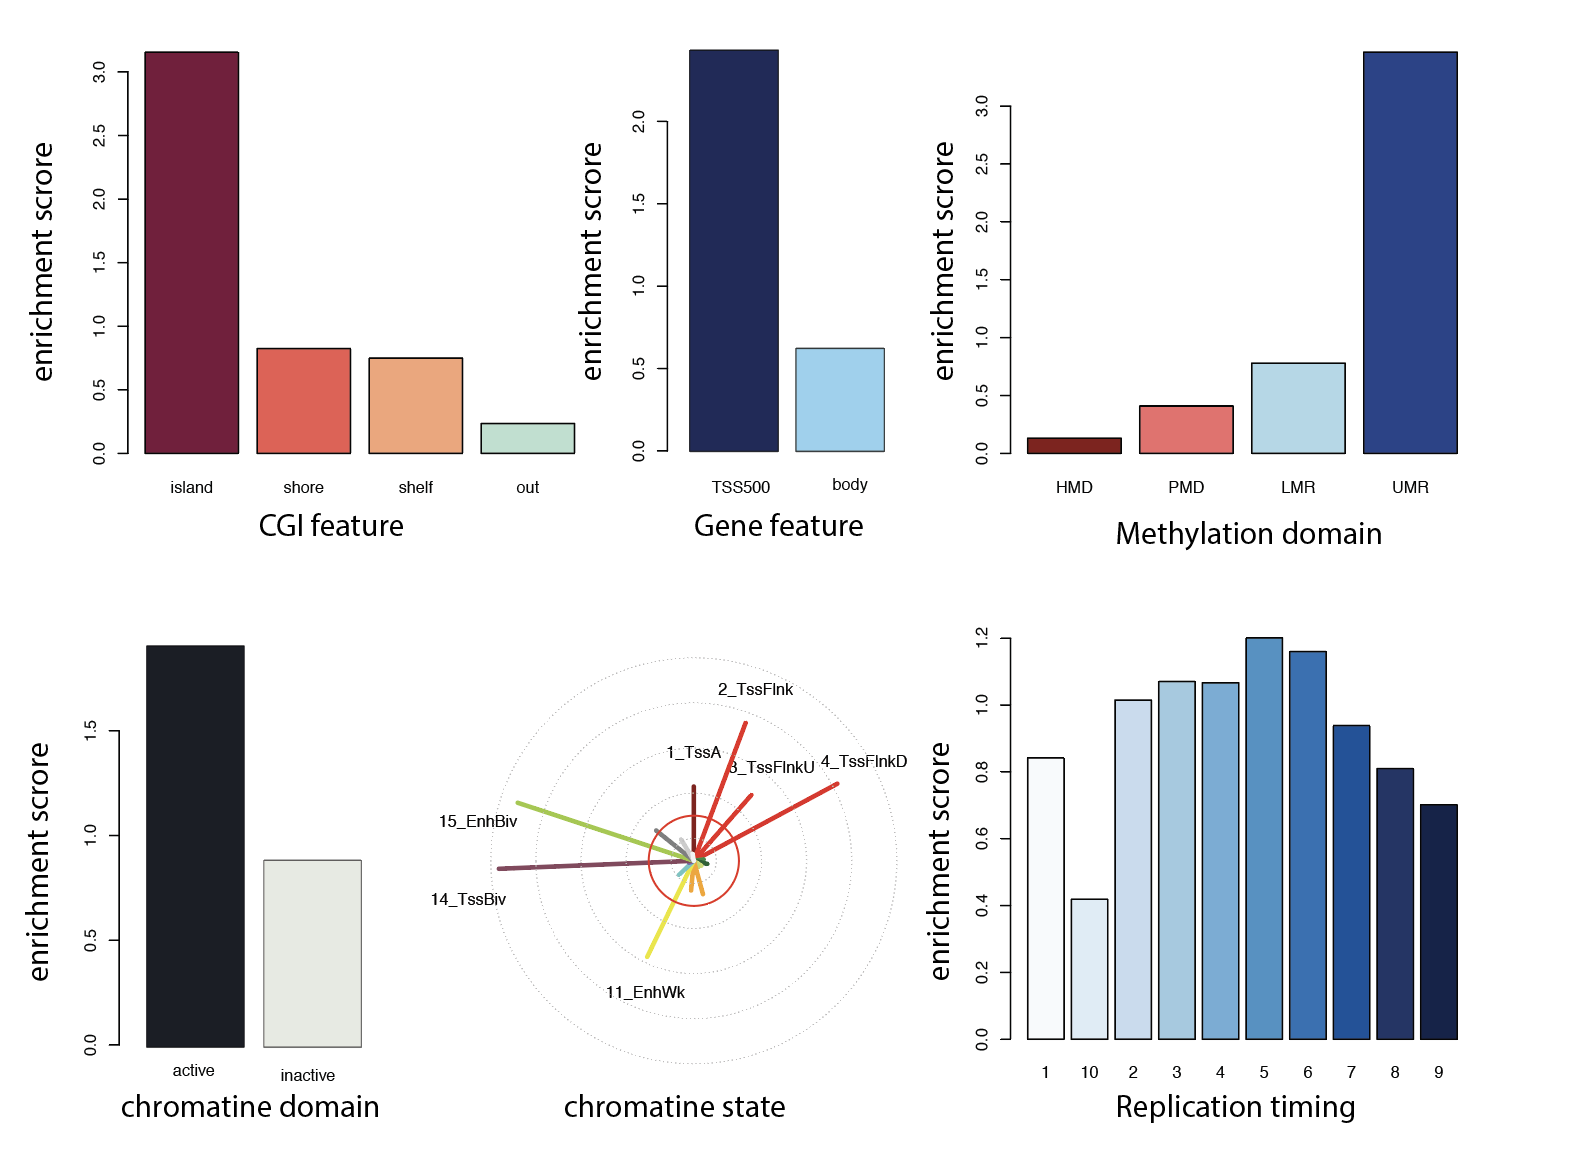
\includegraphics[width=0.8\textwidth,height=0.8\textheight]{./CpG_feature.png}

Zhou et al.~described 48 CpG categories based on the methylation domain,
number of flanking CpG and adjacent nucleotides (Zhou et al., Nat Genet
2018) that are more or less prone to hypomethylation in human tissues.
MethICA allows to annotate these CpG categories, compute and represent
enrichments of MCs most contributing CpG sites within these categories.

\begin{Shaded}
\begin{Highlighting}[]
\CommentTok{# Compute and represent enrichment of 48 CpG categories as in Zhou W et al. (Nat Genet 2018)}
\CommentTok{# create table with categories}
\NormalTok{CpG_feature =}\StringTok{ }\KeywordTok{enrich.CpG.domain}\NormalTok{(}\DataTypeTok{CpG_feature =}\NormalTok{ CpG_feature, }\DataTypeTok{MC_contrib_CpG =}\NormalTok{ MC_contrib_CpG, }\DataTypeTok{MC_active_sample =}\NormalTok{ MC_active_sample)}
\end{Highlighting}
\end{Shaded}

Example of outputs for 48 CpG context in the 20 components:

\begin{figure}
\centering
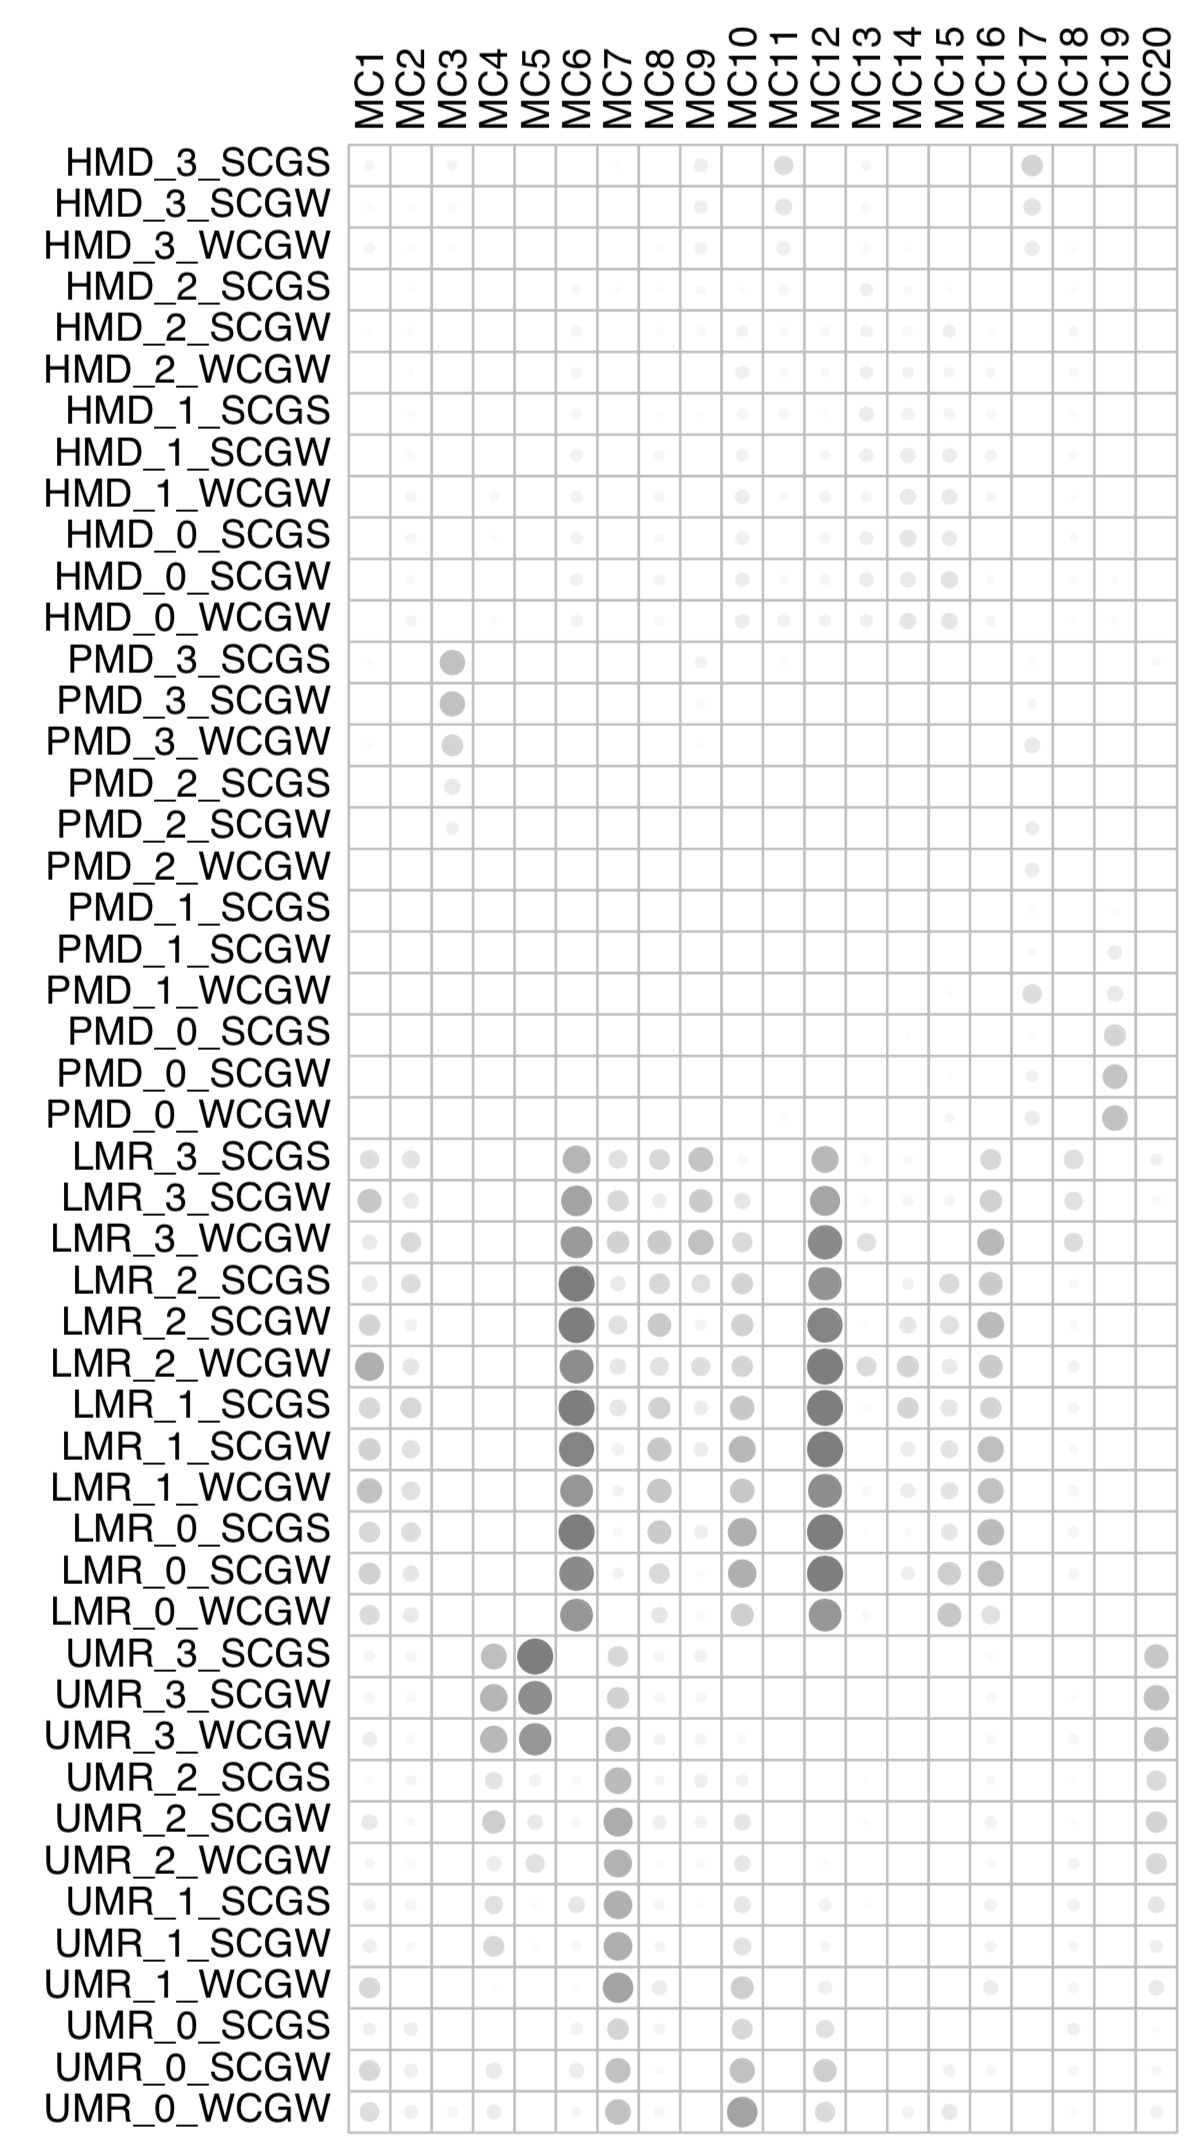
\includegraphics[width=0.4\textwidth,height=0.4\textheight]{./CpG_context_Zhou.png}
\caption{methylation change}
\end{figure}

\hypertarget{association-with-sample-annotations}{%
\section{Association with sample
annotations}\label{association-with-sample-annotations}}

The final step is to analyze the characteristics of samples most
strongly contributing to each component. The mc.annot function first
performs univariate linear regressions to identify annotations
associated with each MC. Significant annotations are then included in
multivariate analyses to determine the strongest determinants of each
MC.

\begin{Shaded}
\begin{Highlighting}[]
\CommentTok{# Association of MCs with clinical and molecular features}
\NormalTok{sample.assoc =}\StringTok{ }\KeywordTok{mc.annot}\NormalTok{(MC_object, }\DataTypeTok{annot =}\NormalTok{ annot , }\DataTypeTok{save =} \OtherTok{TRUE}\NormalTok{, }\DataTypeTok{output.directory =}\NormalTok{ output.directory)}
\end{Highlighting}
\end{Shaded}

Examples of possible representation with this results :

boxplot for one component vs one feature

\begin{Shaded}
\begin{Highlighting}[]
\CommentTok{# Association of MCs with clinical and molecular features}
\KeywordTok{boxplot}\NormalTok{(MC_object}\OperatorTok{$}\NormalTok{Sample_contrib[,}\StringTok{"MC13"}\NormalTok{]}\OperatorTok{~}\StringTok{ }\NormalTok{annot[,}\StringTok{"CTNNB1.alt"}\NormalTok{], }\DataTypeTok{col =} \KeywordTok{c}\NormalTok{(}\StringTok{"grey30"}\NormalTok{, }\StringTok{"grey95"}\NormalTok{), }\DataTypeTok{ylab =} \StringTok{"Sample contribution"}\NormalTok{, }\DataTypeTok{xlab =} \StringTok{"CTNNB1 status"}\NormalTok{, }\DataTypeTok{main =} \StringTok{"MC13 vs CTNNB1 status"}\NormalTok{)}
\end{Highlighting}
\end{Shaded}

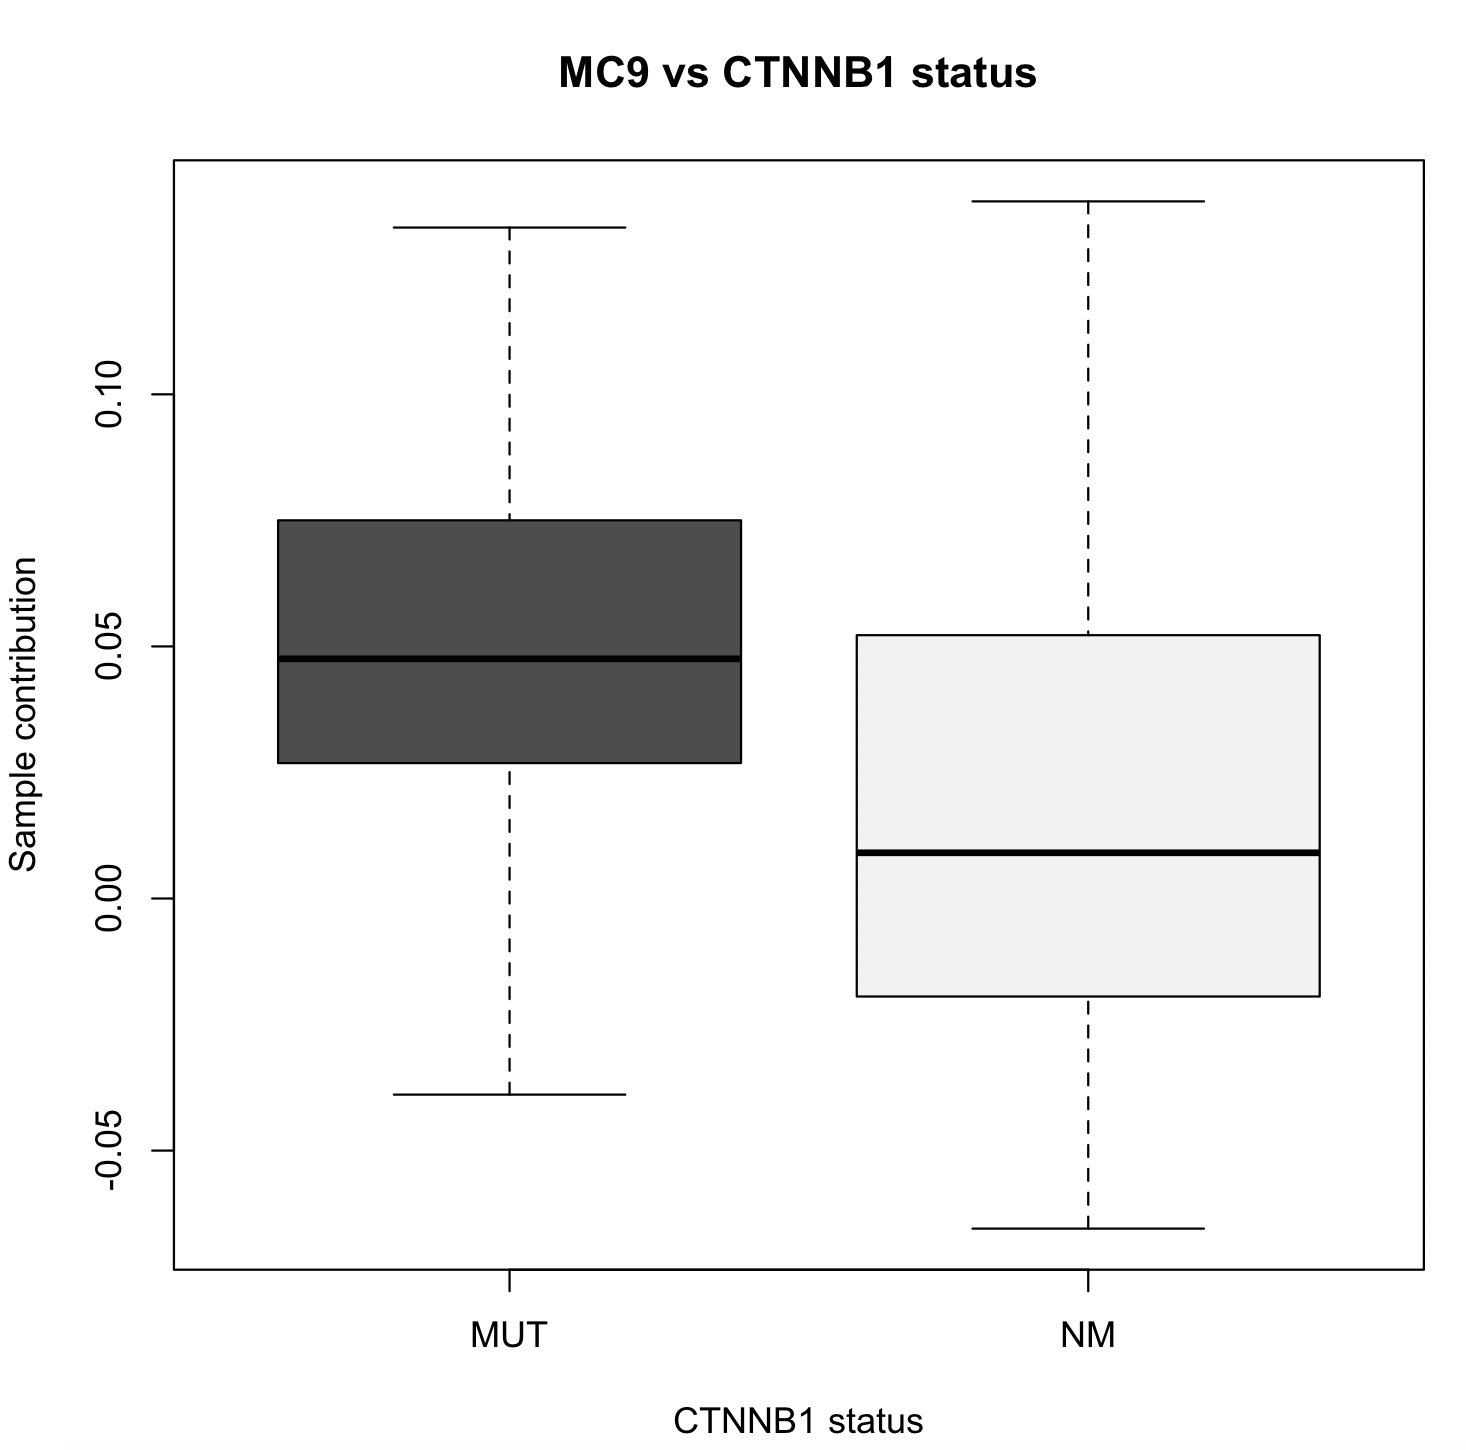
\includegraphics[width=0.3\textwidth,height=0.3\textheight]{./MC9_vs_annot.png}

corrplot of all components vs all features (top = univariate, bottom =
multivariate):

\begin{Shaded}
\begin{Highlighting}[]
\CommentTok{#corrplot representation for univariate and multivariate analyses}
\KeywordTok{association.corrplot}\NormalTok{(}\DataTypeTok{pvaltab_uni =}\NormalTok{ sample.assoc}\OperatorTok{$}\NormalTok{pval_uni , }\DataTypeTok{pvaltab_multi =}\NormalTok{ sample.assoc}\OperatorTok{$}\NormalTok{pval_multi)}
\end{Highlighting}
\end{Shaded}

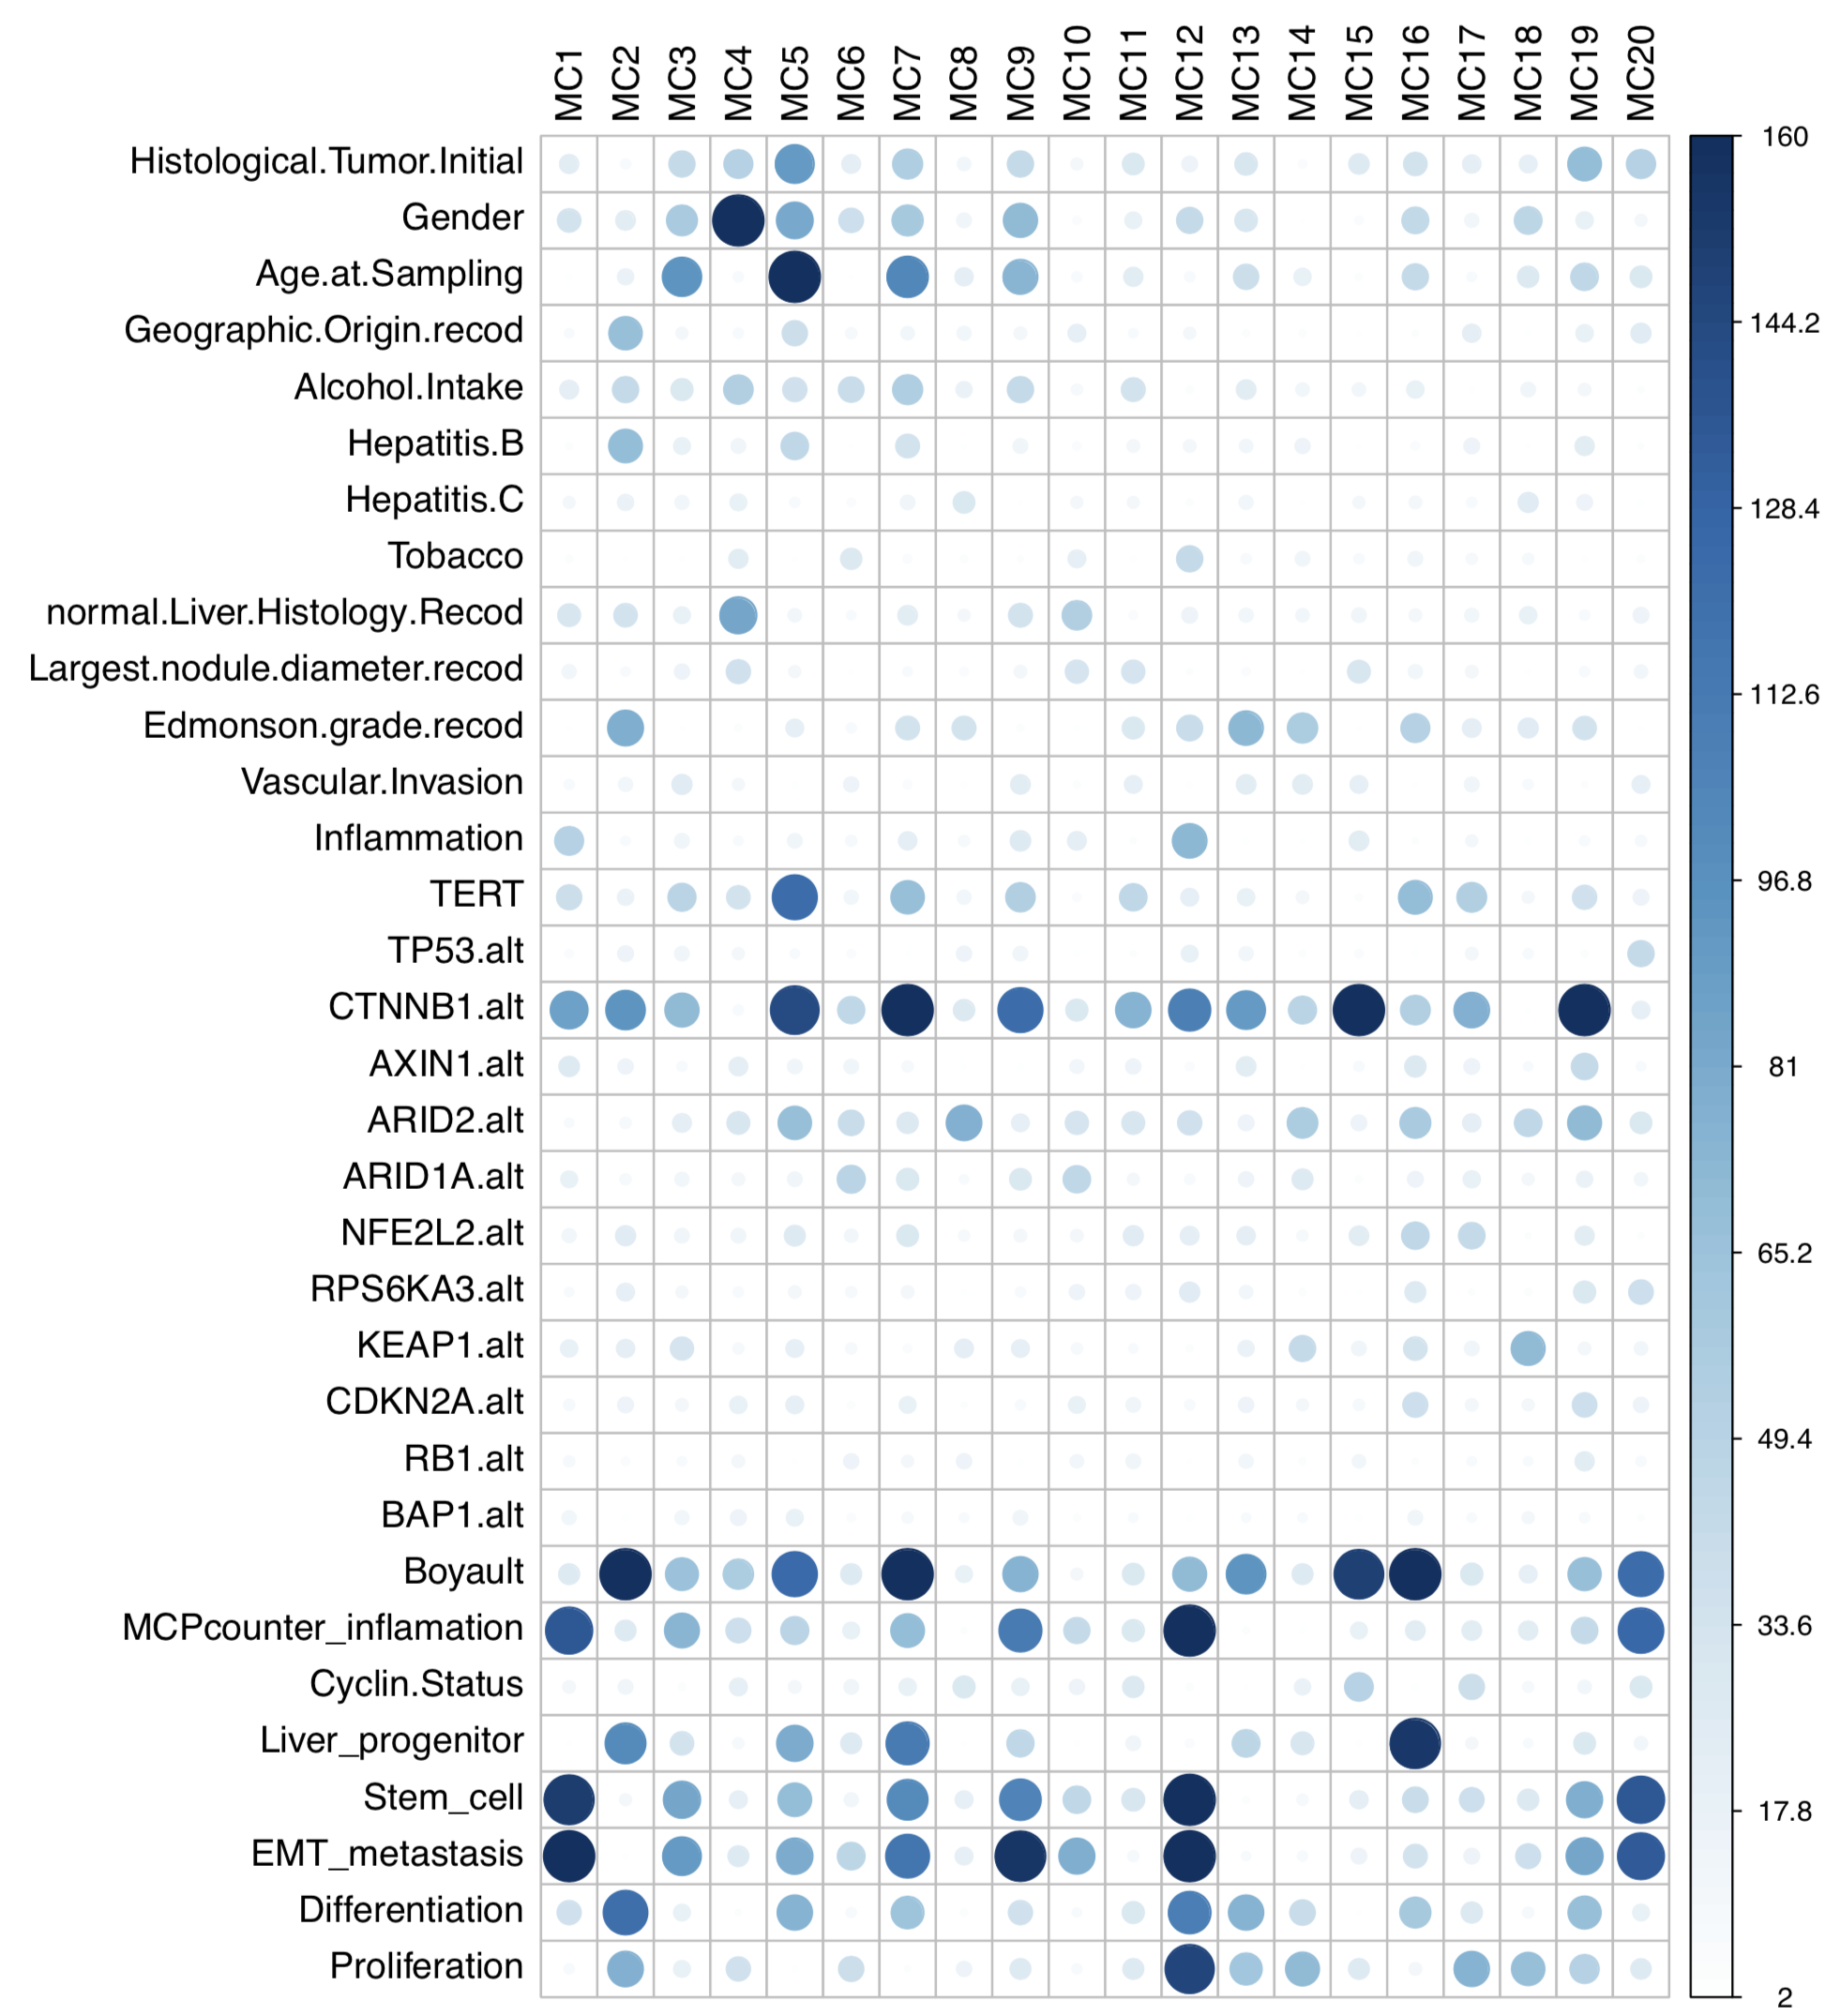
\includegraphics[width=0.6\textwidth,height=0.6\textheight]{./corrplot_uni.png}
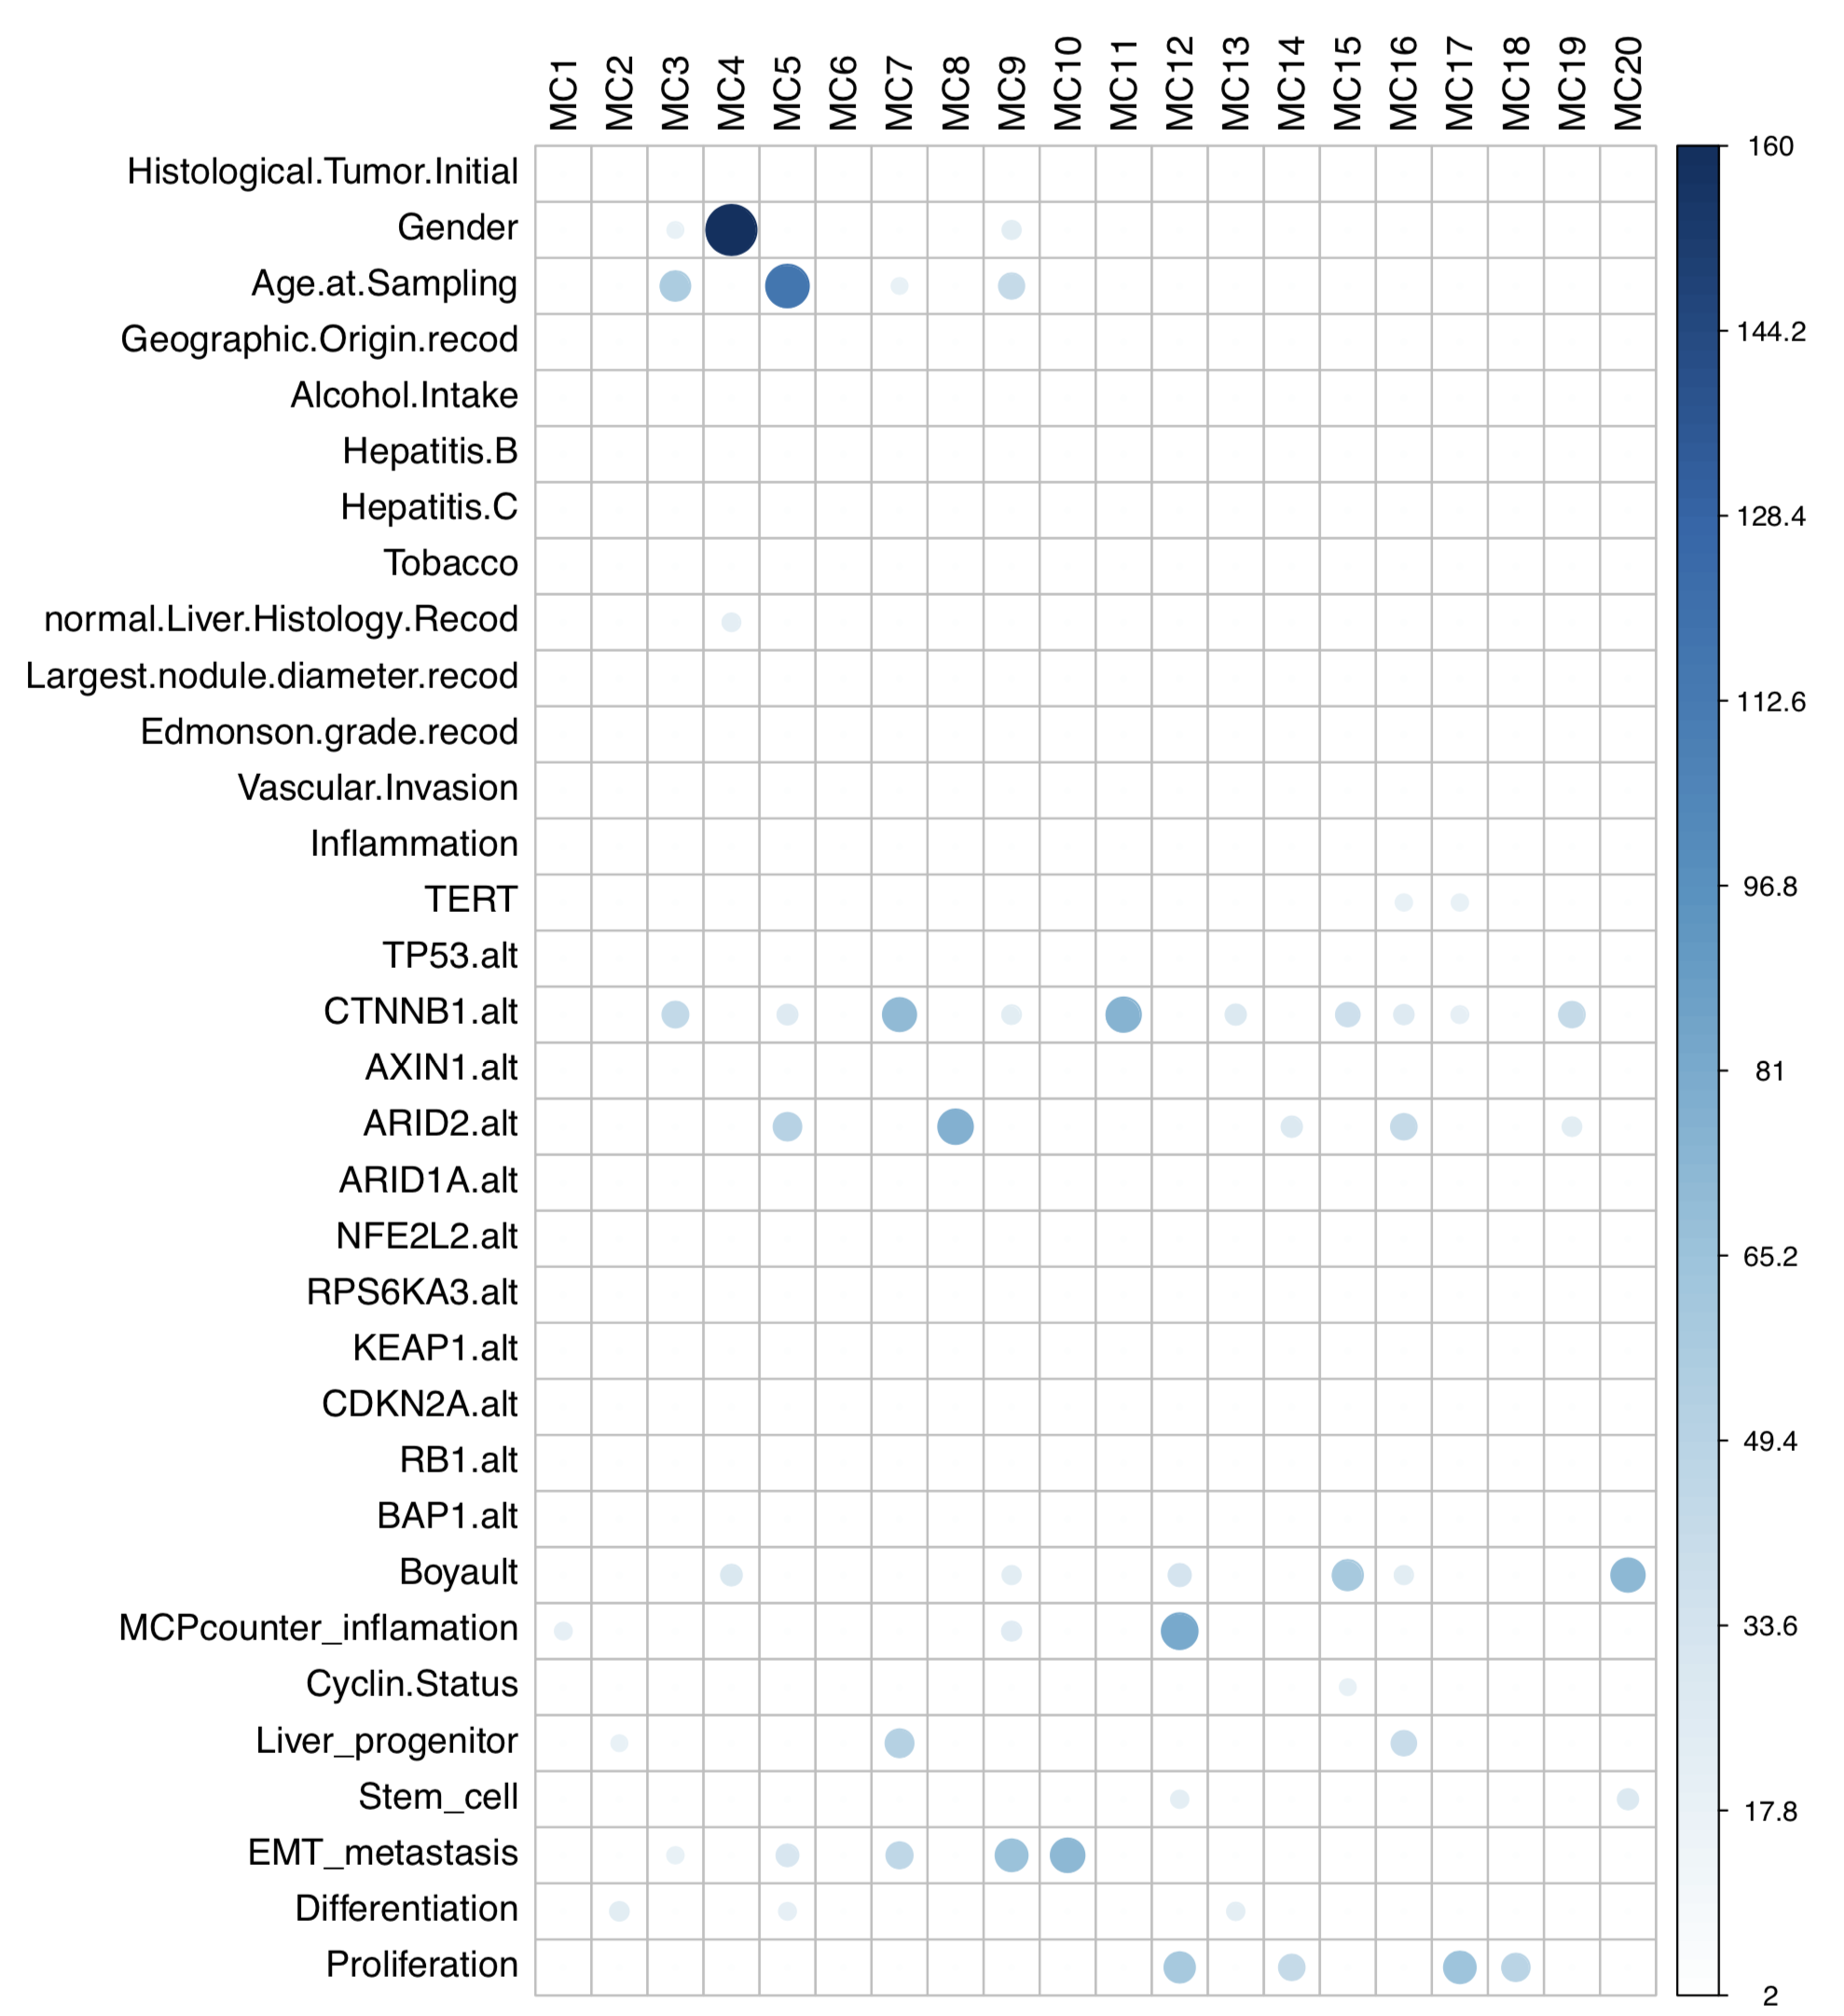
\includegraphics[width=0.6\textwidth,height=0.6\textheight]{./corrplot_multi.png}

p-value circle/color legend (see echelle\_log on the
MethICA\_example\_script.R)

1 = 1

0.1 = 17

0.05 = 22

0.01 = 33

1.0 10-4 = 65

1.0 10-6 = 96

1.0 10-8 = 128

0 = 160

\end{document}
